
\section{\label{sec:Recursion}Prosedur Rekursif\index{rekursi}}

\subsection{Pesulap Matematika}
\begin{lyxlist}{00.00.0000}
\item [{\textsc{Pesulap}}] \textsc{Matematika:} Saya membawa sehelai seprai
biasa. Tidak ada apa-apa di balik lengan baju saya. Tidak ada kantong
rahasia. Mungkin hanya sedikit debu ajaib. Namun selain itu, ini hanyalah
seprai biasa. Ketika dibentangkan rata, tentu saja tebalnya satu lapis.
Saat saya memegang sudut-sudut ini lalu menempatkannya di atas sudut-sudut
yang berseberangan sehingga seprai terlipat menjadi dua, berapa lapiskah
tebalnya?
\item [{\textsc{Penonton:}}] Dua!
\item [{\textsc{Pesulap}}] \textsc{Matematika:} Bagus sekali. Izinkan saya
melipatnya menjadi dua sekali lagi. Sekarang tebalnya menjadi berapa
lapis?
\item [{\textsc{Penonton:}}] Empat!
\item [{\textsc{Pesulap}}] \textsc{Matematika:} Luar biasa. Perhatikan
baik-baik saat saya melipatnya untuk ketiga kalinya. Pikirkan sungguh-sungguh
dan beri tahu saya: sekarang seprai yang terlipat ini tebalnya berapa
lapis?
\item [{\textsc{Penonton:}}] Enam! (dari beberapa orang) Delapan! (dari
lebih banyak orang)
\item [{\textsc{Pesulap}}] \textsc{Matematika:} Betul. Delapan. Cukup sekian
pemanasannya. Sekarang saya akan meminta asisten saya yang menawan
mengeluarkan sehelai seprai biasa lainnya. Kali ini seprai itu sudah
dilipat. Crystal! Tolong bawa seprai itu ... (Crystal membawa seprai
yang sudah dilipat). Sekali lagi, ini seprai biasa. Kali ini sudah
dilipat. Sekarang akan saya lipat menjadi dua seperti sebelumnya,
lalu saya bertanya lagi: seprai ini menjadi berapa lapis?
\item [{\textsc{Penonton:}}] (Sebagian besar diam--hanya terdengar sedikit
gumaman)
\item [{\textsc{Pesulap}}] \textsc{Matematika:} Begitu, rupanya. Yah, saya
juga tidak tahu...
\item [{\textsc{Penonton:}}] (Tertawa)
\item [{\textsc{Pesulap}}] \textsc{Matematika:} ...tetapi saya dapat memberi
tahu Anda bahwa tebalnya sekarang dua kali lipat dari sebelumnya!
\item [{\textsc{Penonton:}}] (Sebagian besar diam--hanya beberapa orang
yang mengerang)
\item [{\textsc{Pesulap}}] \textsc{Matematika:} Saya tahu. Saya tahu. Hanya
trik sulap murahan. Tapi tunggu! Perhatikan saat saya membuka lipatan
seprai ini perlahan-lahan, satu lipatan demi satu. Satu! ... Dua!
(ia menengadah seolah sedang berpikir) ... Tiga! ... (sekali lagi
tampak sedang berpikir keras) ... Empat! ... Setelah empat kali dilipat
menjadi dua, sekarang, seperti yang dapat Anda lihat dengan jelas,
seprai ini tebalnya tiga lapis. Pada lipatan pertama, seprai ini dilipat
menjadi tiga bagian. (ia menatap kejauhan, mengayunkan tongkatnya,
lalu menatap tajam ke mata para penonton) Empat puluh delapan!!!
\item [{\textsc{Penonton:}}] (Diam, tetapi jelas menantikan penjelasan)
\item [{\textsc{Pesulap}}] \textsc{Matematika:} Seprai ini mula-mula tebalnya
3 lapis, lalu ketebalannya digandakan empat kali ... 3 ... 6 ... 12
... 24 ... 48.
\end{lyxlist}
Meskipun dimaksudkan sekadar sebagai celetukan cerdas, pengamatan
bahwa melipat seprai menjadi dua akan menggandakan jumlah lapisan
merupakan kunci untuk menghitung jumlah lapisan pada seprai yang terlipat.
Prosedur rekursif memiliki keajaiban yang sama. Prosedur tersebut
seolah tidak menawarkan sesuatu yang berharga, padahal justru menyimpan
kuncinya. Prosedur tersebut didasarkan pada prinsip bahwa apa pun
keadaan saat ini (berapa pun jumlah lapisan seprai), mengikuti prosedurnya
(melipatnya menjadi dua) akan menghasilkan akibat yang dapat diprediksi
(ketebalannya menjadi dua kali lipat). 

Barangkali contoh numerik paling sederhana dari gagasan ini dapat
dipahami dengan membayangkan sekantong kelereng---kantong tak tembus
pandang yang berisi sejumlah kelereng yang tidak diketahui. Satu kelereng
ditambahkan, lalu Anda ditanya berapa banyak kelereng yang kini ada
di dalamnya. Tentu saja, jawaban terbaik yang dapat Anda berikan kurang
lebih adalah ``satu lebih banyak daripada sebelumnya.'' Walaupun
Anda tidak mengetahui berapa banyak kelereng di dalam kantong pada
awalnya, ketika satu kelereng ditambahkan, Anda tahu bahwa jumlah
yang baru satu lebih banyak daripada jumlah sebelumnya. Inilah cara
berpikir rekursif.

\subsection{Tromino\index{tromino}}

Hubungkan tiga petak persegi, sisi dengan sisi, hingga membentuk huruf
L, dan terbentuklah sebuah tromino. Tromino tidak digunakan dalam
permainan seperti domino, tetapi sering digunakan dalam persoalan
matematika menarik yang melibatkan pengubinan. Mengubin dengan tromino
berarti menutupi suatu bentuk tanpa menumpangtindihkan tromino dan
tanpa membiarkan bagian mana pun dari tromino berada di luar bentuk
yang diubin. Sebagai contoh, kisi $2\times3$ dapat diubin dengan
tromino, demikian pula kisi $6\times9$.
\begin{figure}
\caption{\label{fig:recursion1}$2\times3$ dan $6\times9$ dapat diubin dengan
tromino.}

\centering{}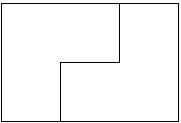
\includegraphics[angle=90]{figures/2x3tiled} 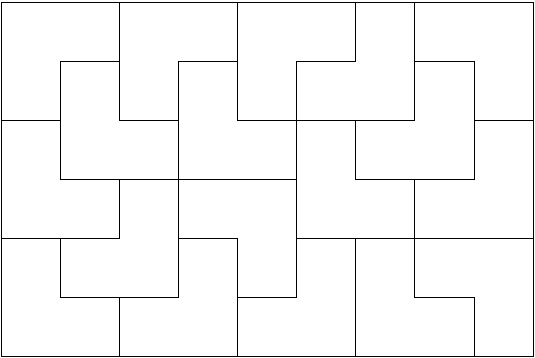
\includegraphics{figures/6x9tiled}
\end{figure}
 Lihat Gambar \ref{fig:recursion1}. Jika $n$ adalah bilangan bulat
positif, kisi $2^{n}\times2^{n}$ hampir dapat diubin seluruhnya dengan
tromino. Semua persegi kecuali satu dapat ditutupi. Cobalah, mula-mula
dengan kisi $2\times2$. Yang ini tidak terlalu sulit. Kemudian cobalah
dengan kisi $4\times4$ atau kisi $8\times8$.

Bagaimana dengan kisi $1024\times1024$? Saya tidak menyarankan Anda
benar-benar menyiapkan kisi $1024\times1024$ lalu mulai mengisinya
dengan tromino. Anda akan memerlukan $349,525$ tromino. Anda mungkin
tidak akan menyelesaikannya seumur hidup! Sebagai gantinya, sekarang
saatnya mulai berpikir secara rekursif. Gunakan hasil sebelumnya dalam
jawaban Anda. Seperti ketika Anda cukup mengatakan bahwa kantong kelereng
``berisi satu lebih banyak daripada sebelumnya'', kita dapat menyatakan
solusi pengubinan kisi $1024\times1024$ berdasarkan pengubinan kisi
$512\times512$. Caranya sebagai berikut. Ambil kisi $1024\times1024$
dan bagi menjadi empat subkisi $512\times512$ dengan membelahnya
di tengah secara horizontal dan vertikal. Pada kisi $512\times512$
di kiri atas, ubin semua persegi kecuali sudut kanan bawah. Pada kisi
$512\times512$ di kiri bawah, ubin semua persegi kecuali sudut kanan
atas. Pada kisi kanan bawah, ubin semua persegi kecuali sudut kiri
atas. Terakhir, pada kisi $512\times512$ di kanan atas, ubin semua
persegi kecuali sudut kanan atas 
\begin{figure}
\caption{\label{fig:recursion2} Kisi $2^{n}\times2^{n}$ dapat (hampir) diubin
secara rekursif.}

\centering{}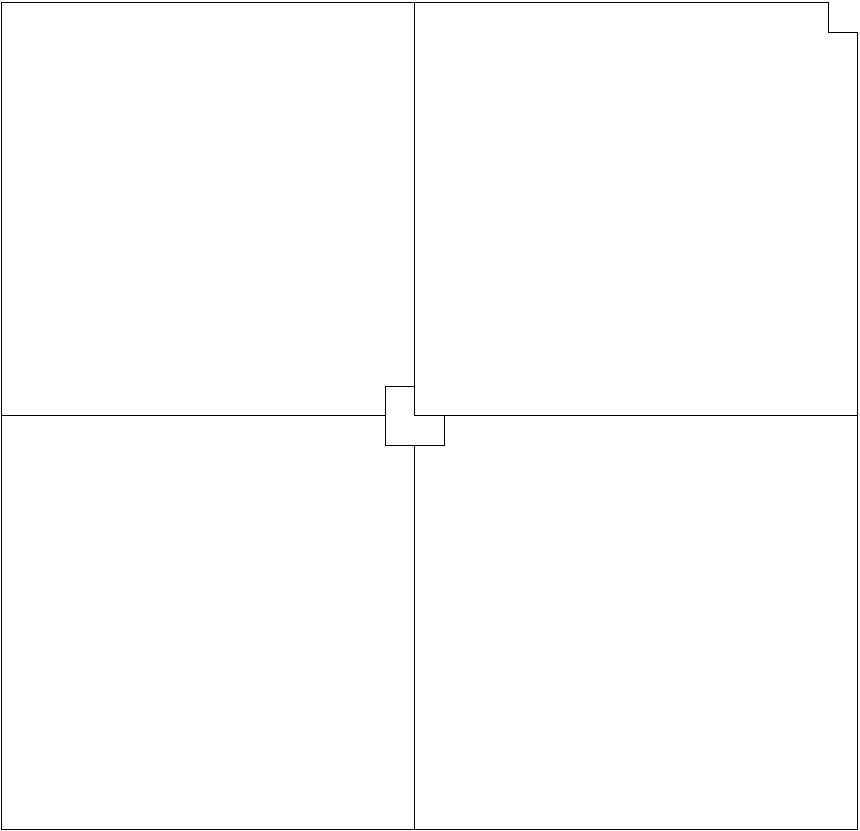
\includegraphics[scale=0.5]{figures/recursiveTiling}
\end{figure}
(Gambar \ref{fig:recursion2}). Hal ini menyisakan ruang untuk satu
tromino berbentuk L di tengah dan satu persegi yang tidak tertutupi.
Selesai! Cara ini mungkin terasa sedikit curang karena kita tidak
menjelaskan cara menangani kisi $512\times512$; namun, argumen yang
sama berlaku untuk kisi $512\times512$. Anda dapat membaginya menjadi
empat subkisi, mengubin semuanya, dan selesai.

Argumen pengubinan yang sama dapat diterapkan pada setiap kisi $2^{n}\times2^{n}$
berdasarkan pengubinan kisi $2^{n-1}\times2^{n-1}$, kecuali ketika
$n=1$. Anda hanya perlu mengubin sendiri kisi $2\times2$! Setelah
itu selesai, Anda memperoleh solusi lengkap untuk setiap kisi $2^{n}\times2^{n}$.
\begin{figure}
\caption{\label{fig:recursion3} Kisi $32\times32$ yang diubin secara rekursif.}

\centering{}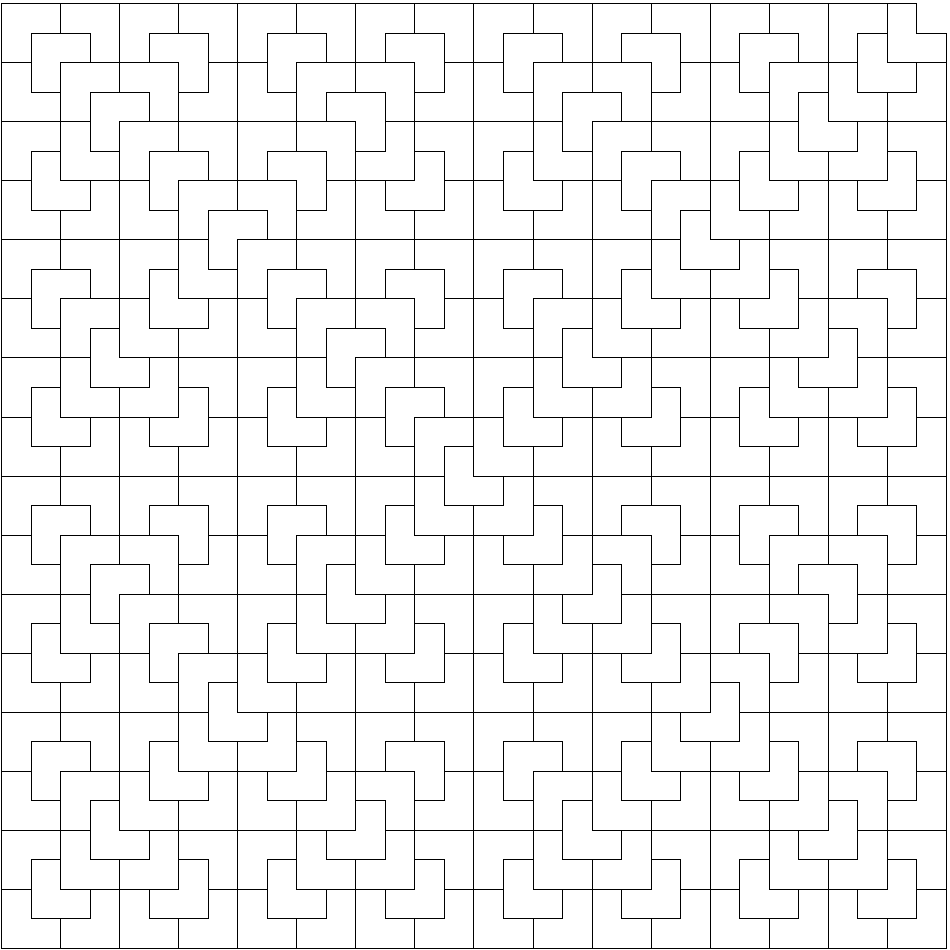
\includegraphics[scale=0.5]{figures/32x32recursive}
\end{figure}
Pengecualian serupa berlaku bagi setiap prosedur rekursif. Rekursi
hanya berguna pada hampir semua tahap. Pada suatu titik, Anda harus
turun tangan dan memberikan solusi atau jawaban. Jawaban semacam itu
sering disebut kondisi awal.

\begin{digression}{Pembuktian dengan induksi} 

\noindent Pembuktian dengan induksi juga menggunakan semacam cara
berpikir rekursif. Dalam metode ini, kita harus membuktikan bahwa
suatu klaim benar untuk suatu nilai variabel. Bagian ini serupa dengan
memiliki kondisi awal. Selanjutnya, harus dibuktikan bahwa kebenaran
klaim untuk nilai $n$ mengakibatkan kebenaran klaim untuk $n+1$.
Hal ini serupa dengan hubungan rekursif antarkeadaan. Bahkan, konstruksi
pengubinan kisi $2^{n}\times2^{n}$ berdasarkan kisi $2^{n-1}\times2^{n-1}$
ditambah pengubinan kisi $2\times2$ yang baru saja disajikan pada
dasarnya membentuk pembuktian dengan induksi bahwa kisi $2^{n}\times2^{n}$,
kecuali satu sudutnya, dapat diubin dengan tromino untuk setiap $n\geq1$.
Dengan demikian, semua pembuktian dengan induksi pada akhirnya bergantung
pada kemampuan melihat hubungan rekursif antarkeadaan.

Pada tahun 1954, Solomon Golomb \index{Golomb!Solomon} menerbitkan
pembuktian dengan induksi bahwa kisi $2^{n}\times2^{n}$ yang kehilangan
satu persegi \textit{sembarang} (tidak harus petak sudut), yang disebut
persegi defisien, dapat diubin dengan tromino. Dapatkah Anda menyusun
pengubinan (rekursif) untuk persegi defisien $2^{n}\times2^{n}$?
Dalam konstruksi tersebut, Anda dapat menggunakan pengubinan kisi
$2^{k}\times2^{k}$ yang dikurangi satu sudut.
\begin{description}
\item [{Referensi}] \cite{golomb}
\end{description}
\end{digression}

\subsection{Octave}

\subsubsection{Fungsi buatan sendiri\index{Octave!fungsi buatan sendiri}}

Seperti bahasa pemrograman modern yang berguna pada umumnya, Octave
memungkinkan kita membuat fungsi sendiri, tidak hanya fungsi yang
dapat ditulis sebagai rumus satu baris seperti fungsi anonim. Misalkan
Anda ingin menentukan nilai maksimum suatu fungsi pada sekumpulan
nilai yang berjarak sama. Fungsi itu memiliki tujuan yang sangat khusus
dan jarang digunakan. Oleh karena itu, fungsi tersebut tidak tersedia
sebagai bawaan dalam bahasa pemrograman mana pun; jika benar-benar
menginginkannya, Anda perlu menulisnya sendiri. Demikian pula, jika
Anda menginginkan fungsi yang menghitung titik simedian suatu segitiga,
Anda perlu menulisnya. Bahkan, hampir semua komputasi di luar evaluasi
fungsi dasar tidak tersedia sebagai bawaan di Octave.

Fungsi buatan sendiri ditulis berdasarkan tiga informasi pokok: nama
fungsi, daftar masukan, dan uraian keluaran. Ketiganya harus ditetapkan
dengan jelas sebelum fungsi mulai ditulis. Untuk menulis fungsi, kita
hanya perlu memberi tahu Octave nama dan masukan yang diinginkan serta
cara menentukan keluarannya. Format dasar suatu fungsi adalah sebagai
berikut:\begin{verbatim}
function ans = myName(input1, input2, ... )
  ...
  ans = final answer;
end%function
\end{verbatim}Baris pertama memuat nama fungsi dan daftar masukan. Bagian fungsi
lainnya digunakan untuk menghitung keluaran, \texttt{ans}.

Fungsi yang menentukan nilai maksimum suatu fungsi pada sekumpulan
nilai yang berjarak sama dapat ditulis melalui langkah-langkah berikut.
Pertama, kita memutuskan untuk menamainya ``maxOverMesh''. Perhatikan
bahwa nama tersebut tidak mengandung spasi atau karakter khusus. Hanya
sedikit karakter nonalfabet yang dapat digunakan dalam nama fungsi.
Biasanya tanda garis bawah dan angka aman digunakan, tetapi karakter
lain belum tentu dapat digunakan! Sebaiknya batasi diri pada karakter
tersebut. Kedua, kita perlu memikirkan masukan yang diperlukan fungsi
ini. Tentu saja, fungsi yang akan dimaksimumkan diperlukan, dan kisi
titik tempat fungsi itu diperiksa juga harus ditentukan. Ada beberapa
cara untuk melakukannya, tetapi cara yang mungkin paling mudah bagi
pengguna ialah meminta titik ujung bawah, titik ujung atas, dan jumlah
interval pada kisi. Terakhir, kita perlu menulis kode yang menerima
masukan tersebut dan menentukan nilai maksimum fungsi pada kisi. Salah
satu caranya adalah sebagai berikut: \begin{verbatim}
%%%%%%%%%%%%%%%%%%%%%%%%%%%%%%%%%%%%%%%%%%%%%%%%%%%%%%%%%%%
%  maxOverMesh() written by Leon Q. Brin 21 January 2013  %
%  INPUT: Interval [a,b]; function f; and number of       %
%         subintervals n.                                 %
%  OUTPUT: maximum value of the function over the end     %
%         points of the subintervals.                     %
%%%%%%%%%%%%%%%%%%%%%%%%%%%%%%%%%%%%%%%%%%%%%%%%%%%%%%%%%%% 
function ans = maxOverMesh(f,a,b,n)
  ans = f(a);
  for i=1:n
    x = (i*b + (n-i)*a)/n;
    F = f(x);
    if (F>ans) ans = F;
  end%for
end%function
\end{verbatim}Merupakan praktik yang baik untuk mengawali setiap fungsi yang Anda
tulis dengan komentar berisi uraian tiga hal tentang fungsi tersebut---nama,
masukan, dan keluaran. Jika kelak Anda atau orang lain membacanya,
tersedia ringkasan singkat tentang cara dan tujuan penggunaan fungsi
tersebut.

Nilai yang disimpan dalam \texttt{ans} saat fungsi selesai menjadi
keluaran fungsi. Pada awalnya, \texttt{ans} diisi dengan nilai fungsi
di titik ujung kiri. Selanjutnya, fungsi melakukan perulangan melalui
titik-titik ujung subselang lainnya dan menghitung nilai fungsi pada
setiap titik. Setiap kali menemukan nilai yang lebih besar daripada
\texttt{ans}, fungsi memperbarui nilai \texttt{ans} dengan nilai tersebut.
Pada akhir perulangan, \texttt{ans} berisi nilai terbesar fungsi.

Untuk menggunakan fungsi buatan sendiri, simpan fungsi tersebut dalam
berkas \texttt{.m} \index{Octave!berkas .m@berkas \texttt{.m}} dengan
nama yang sama dengan nama fungsi. Sebagai contoh, fungsi \texttt{maxOverMesh()}
akan disimpan dalam berkas bernama \texttt{maxOverMesh.m}. Setelah
itu, fungsi buatan sendiri dapat dipanggil seperti fungsi bawaan Octave
mana pun, asalkan berkas \texttt{.m} dan program yang menggunakannya
disimpan dalam direktori yang sama. Jika fungsi digunakan dari baris
perintah, direktori kerja Octave (direktori tempat Octave dijalankan,
kecuali diubah secara eksplisit selama sesi) harus merupakan direktori
tempat berkas \texttt{.m} disimpan:\begin{verbatim}
octave:1> maxOverMesh(@(x) (x^2-6*x+8)*exp(x), 0, 4, 99)
ans =  8.6728
octave:2> f = @(x) (x^2+3*x-5)/(x^2-3*x+5)
f =
@(x) (x ^ 2 + 3 * x - 5) / (x ^ 2 - 3 * x + 5)
octave:3> maxOverMesh(f, -5, 5, 225)
ans =  2.6362
\end{verbatim}\texttt{maxOverMesh.m} dapat diunduh dari \href{http://lqbrin.github.io/tea-time-numerical/ancillaries.html}{situs pendamping}.

\subsubsection{Fungsi rekursif}

Dengan berpikir secara rekursif, apa jawaban Anda jika saya menanyakan
nilai $10!$? Renungkan sejenak sebelum melanjutkan. Betul! 10 faktorial
hanyalah 10 dikalikan $9!$:
\begin{eqnarray*}
10! & = & 10\cdot9\cdot8\cdot7\cdot6\cdot5\cdot4\cdot3\cdot2\cdot1\\
 & = & 10\cdot(9\cdot8\cdot7\cdot6\cdot5\cdot4\cdot3\cdot2\cdot1)\\
 & = & 10\cdot(9!).
\end{eqnarray*}
Tidak perlu memperoleh sebuah bilangan. Cukup gunakan gagasan rekursif,
sebab gagasan itu tentu sama berlakunya untuk $9!$, dan seterusnya
$\ldots$ hingga (atau mungkin seharusnya saya katakan menurun hingga?)
suatu titik. Pada titik apa pernyataan $n!=n\cdot(n-1)!$ tidak lagi
benar? Ketika $n=0$. Kita perlu menetapkan bahwa $0!=1$ dan tidak
mengandalkan pemikiran rekursif dalam kasus ini. Namun, hanya dalam
kasus ini!

Mari kita lihat bagaimana perhitungan rekursif ini bekerja untuk $5!$.
Menurut rekursi tersebut, $5!=5\cdot4!$. Namun, $4!=4\cdot3!$ sehingga
diperoleh $5!=5\cdot(4\cdot3!)$. Namun, $3!=3\cdot2!$ sehingga sekarang
diperoleh $5!=5(4(3\cdot2!))$. Dengan melanjutkan proses ini, $2!=2\cdot1!=2\cdot1\cdot0!$
sehingga sekarang diperoleh $5!=5(4(3(2(1\cdot0!))))$. Sekarang rekursi
berhenti dan kita cukup menyubstitusikan 1 untuk $0!$ sehingga diperoleh
$5!=5(4(3(2(1(1)))))$. Mungkin Anda mengharapkan $5\cdot4\cdot3\cdot2\cdot1$
sebagai hasil akhirnya. Tentu saja, kedua cara tersebut sama-sama
menghasilkan 120, sehingga dari segi ketepatan, keduanya tidak bermasalah.
Secara praktis, perbedaannya tidak berarti. Menghitung faktorial secara
rekursif amat tidak efisien dan mustahil dilakukan melampaui kedalaman
rekursi maksimum bahasa pemrograman yang digunakan, sehingga cara
ini tidak boleh dipakai dalam praktik. Satu-satunya manfaatnya adalah
sebagai latihan berpikir dan memprogram secara rekursif.

Secara umum, fungsi rekursif \index{Octave!fungsi rekursif} akan
tampak seperti berikut:\begin{verbatim}
function ans = recFunction(input1, input2, ... )
  if (recursion does not apply)
    return appropriate ans
  else
    return recFunction(i1, i2, ... )
  end%if
end%function
\end{verbatim}Hal pertama yang perlu dilakukan adalah menentukan apakah rekursi
berlaku. Jika tidak, keluaran yang sesuai harus diberikan. Jika ya,
fungsi rekursif cukup memanggil dirinya sendiri dengan masukan yang
telah diubah. Karena definisi rekursif (yang agak usil) untuk $n!$
adalah $n\cdot(n-1)!$ dan berlaku setiap kali $n>0$, sedangkan $0!=1$,
fungsi faktorial rekursif dapat tampak seperti berikut:\begin{verbatim}
%%%%%%%%%%%%%%%%%%%%%%%%%%%%%%%%%%%%%%%%%%%%%%%%%%%%%%%%%%%%
%  recFactorial() written by Leon Q. Brin 21 January 2013  %
%       is a recursively defined factorial function.       %
%  INPUT: nonnegative integer n.                           %
%  OUTPUT: n!                                              %
%%%%%%%%%%%%%%%%%%%%%%%%%%%%%%%%%%%%%%%%%%%%%%%%%%%%%%%%%%%%
function ans = recFactorial(n)
  if (n==0)
    ans = 1;
  else
    ans = n*recFactorial(n-1);
  end%if
end%function
\end{verbatim}

\noindent Perhatikan \texttt{==} ketika memeriksa apakah \texttt{n}
sama dengan \texttt{1}. Ini bukan kesalahan ketik. Hal ini sangat
penting. Semua bahasa pemrograman harus membedakan penugasan dan kondisi.
Di atas kertas, menuliskan $x=3$ ketika Anda ingin menetapkan $x$
sama dengan 3 mungkin terasa wajar. Menuliskan ``jika $x=3$, semuanya
baik-baik saja'' juga mungkin terasa wajar. Kita menggunakan ``persamaan''
$x=3$ dengan cara yang persis sama di atas kertas untuk menyatakan
dua hal yang sangat berbeda. Ketika kita menetapkan $x=3$ kita membuat
sebuah pernyataan, atau melakukan penugasan nilai 3 kepada variabel
$x$. Namun, ketika kita menulis ``jika $x=3\ldots$'' kita membuat
pernyataan hipotetis, atau pernyataan kondisional. Nilai $x$ belum
diketahui. Dalam Octave, keduanya dibedakan dengan menggunakan satu
tanda sama dengan, \texttt{=}, untuk menyatakan penugasan dan dua
tanda sama dengan, \texttt{==}, untuk menguji kesamaan. Operator perbandingan
lain yang mungkin Anda perlukan adalah \texttt{<} dan \texttt{>},
yang memiliki arti sebagaimana lazimnya, serta \texttt{<=} dan \texttt{>=}
yang masing-masing berarti $\leq$ dan $\geq$, secara berurutan.
\texttt{recFactorial.m} dapat diunduh dari \href{http://lqbrin.github.io/tea-time-numerical/ancillaries.html}{situs pendamping}.

\noindent\startexercises

\subsection{Latihan}
\begin{enumerate}
\item \octave\ Tulislah berkas .m dengan sebuah fungsi yang menerima satu
masukan, menguadratkannya, dan mengembalikan hasilnya. Berkas Anda
harus

\begin{enumerate}
\item memuat blok komentar di bagian awal yang berisi nama Anda, tanggal,
serta penjelasan mengenai apa yang dilakukan program tersebut dan
cara menggunakannya.
\item memuat fungsi berbentuk \texttt{foo(x)} yang mengembalikan kuadrat
dari masukan (argumen) \texttt{x}.
\end{enumerate}
Pastikan Anda menguji fungsi tersebut melalui baris perintah Octave.
\item \octave\ Fungsi Octave \texttt{foo(x)} ditampilkan di bawah ini.

\begin{verbatim}
function res = foo(x)
  if (x<1)
    res = 0;
  else
    half = x/2;
    floorhalf = floor(half);
    if (half == floorhalf)
      res = 0 + foo(floorhalf);
    else
      res = 1 + foo(floorhalf);
    end%if
  end%if
end%function
\end{verbatim}
\begin{enumerate}
\item Hitung \texttt{foo(2)}.
\item Hitung \texttt{foo(23)}.
\end{enumerate}
\item \octave\ Tulislah fungsi Octave rekursif yang menghitung 
\[
\sum_{i=1}^{n}\frac{1}{i}
\]
\item \octave\ Tulislah fungsi Octave rekursif yang menghitung $a_{n}$
untuk setiap $n\geq0$, dengan ketentuan
\begin{eqnarray*}
a_{0} & = & 100,000\\
a_{n} & = & 1.05a_{n-1}-1200,\quad n>0.
\end{eqnarray*}
\item \label{recursive1}Barisan Fibonacci, $\left\langle F_{n}\right\rangle $,
didefinisikan secara rekursif oleh
\begin{align*}
F_{n+1} & =F_{n}+F_{n-1},\quad n\geq1\\
F_{0} & =1\\
F_{1} & =1
\end{align*}
sehingga beberapa suku pertamanya adalah $1,1,2,3,5,8$. 

\begin{enumerate}
\item \label{recursiveFib}Tulislah fungsi rekursif yang menghitung suku
$n$ dalam barisan Fibonacci. Fungsi Anda harus memiliki satu argumen,
$n$. 
\item \label{forloopFib}Tulislah fungsi yang menggunakan perulangan for
untuk menghitung suku $n$ dalam barisan Fibonacci. Fungsi Anda harus
memiliki satu argumen, $n$. 
\item Tulislah program yang memanggil fungsi dari \ref{recursiveFib} untuk
menghitung $F_{30}$.
\item Tulislah program yang memanggil fungsi dari \ref{forloopFib} untuk
menghitung $F_{30}$.
\item Kode manakah yang lebih sederhana (rekursif atau nonrekursif)?
\item Kode manakah yang lebih cepat?
\item Kode manakah yang lebih akurat?
\end{enumerate}
\textbf{CATATAN}: $F_{30}=1346269$.
\item \label{recursive2}Misalkan barisan $\left\langle a_{n}\right\rangle $
didefinisikan oleh 
\begin{align*}
a_{n+1} & =\frac{1}{4}\left|5a_{n}^{2}-30a_{n}+25\right|,\quad n\geq1\\
a_{0} & =\frac{17+2\sqrt{7}}{5}.
\end{align*}

\begin{enumerate}
\item Hitung $a_{1},a_{2}$ dan $a_{3}$ secara eksak.
\item Tentukan $a_{20}$ dan $a_{51}$ secara eksak.
\item Tulislah fungsi rekursif yang menghitung suku $n$ dari barisan tersebut.
Fungsi Anda harus memiliki satu argumen, $n$. Tulislah program yang
memanggil fungsi ini untuk menghitung $a_{1},a_{2},a_{3},a_{20},$
dan $a_{51}$.
\item Tulislah fungsi yang menggunakan perulangan for untuk menghitung suku
$n$ dari barisan tersebut. Fungsi Anda harus memiliki satu argumen,
$n$. Tulislah program yang memanggil fungsi ini untuk menghitung
$a_{1},a_{2},a_{3},a_{20},$ dan $a_{51}$.
\item Kode manakah yang lebih sederhana (rekursif atau nonrekursif)?
\item Fungsi manakah yang lebih cepat?
\item Kode manakah yang lebih akurat, dan mengapa?
\item Fungsi manakah yang lebih baik, dan mengapa?
\item Apakah Anda yakin salah satu dari kedua fungsi tersebut dapat menghitung
$a_{600}$ secara akurat? Jika tidak, mengapa?
\end{enumerate}
\item \label{exc:recursion}Tromino, bagian 1. \hasananswer 

\begin{enumerate}
\item Dengan pendekatan rekursif, berapa banyak tromino yang diperlukan
untuk mengubin kisi $2^{n}\times2^{n}$ dengan menyisakan satu persegi
di sudut?
\item \label{tromino-greatest}Berapa nilai bilangan bulat terbesar untuk
$n$ yang tidak tercakup dalam definisi rekursif tersebut?
\item Untuk nilai $n$ pada bagian \ref{tromino-greatest}, berapa banyak
tromino yang diperlukan?
\end{enumerate}
\item \label{exc:recursion-1}\octave\ Tromino, bagian 2. \hasasolution 

\begin{enumerate}
\item Tulislah fungsi Octave rekursif untuk menghitung banyaknya tromino
yang diperlukan untuk mengubin kisi $2^{n}\times2^{n}$ dengan menyisakan
satu persegi di sudut.
\item Gunakan fungsi Anda untuk memverifikasi bahwa sebanyak $349,525$
tromino diperlukan untuk mengubin kisi $1024\times1024$ dengan menyisakan
satu persegi di sudut.
\end{enumerate}
\item \label{exc:recursion-2}Menara Hanoi, bagian 1. Menara Hanoi adalah
permainan yang menggunakan sejumlah cakram dengan ukuran berbeda-beda,
yang ditumpuk pada sebuah tiang dari yang terbesar di bawah hingga
yang terkecil di atas. Terdapat dua tiang lain yang pada awalnya kosong.
Tujuannya adalah memindahkan seluruh tumpukan cakram ke salah satu
tiang yang semula kosong dengan mengikuti dua aturan. Anda hanya boleh
memindahkan satu cakram pada satu waktu dari satu tiang ke tiang lain.
Anda tidak boleh meletakkan cakram di atas cakram yang lebih kecil. \hasasolution 

\begin{enumerate}
\item Dengan memulai dari tumpukan tiga cakram, berapakah jumlah langkah
minimum yang diperlukan untuk menyelesaikan permainan? Jawablah pertanyaan
ini dengan sebuah bilangan.
\item Dengan memulai dari tumpukan empat cakram, berapakah jumlah langkah
minimum yang diperlukan untuk menyelesaikan permainan?

\begin{enumerate}
\item \label{enu:tower-recursion}Jawablah pertanyaan ini secara rekursif.
\item Berdasarkan jawaban rekursif Anda, jawablah pertanyaan ini dengan
sebuah bilangan.
\end{enumerate}
\end{enumerate}
\item \label{exc:recursion-3}Menara Hanoi, bagian 2. \hasasolution 

\begin{enumerate}
\item Dengan memulai dari sebuah ``tumpukan'' yang hanya terdiri dari
satu cakram, berapakah jumlah langkah minimum yang diperlukan untuk
menyelesaikan permainan?
\item \octave\ Gunakan jawaban Anda untuk bagian (a), bersama generalisasi
jawaban Anda atas soal  \ref{enu:tower-recursion} untuk menulis fungsi
Octave rekursif yang menghitung jumlah langkah minimum yang diperlukan
untuk menyelesaikan permainan dengan tumpukan $n$ cakram.
\item \octave\ Gunakan fungsi Octave Anda untuk memverifikasi bahwa jumlah
langkah minimum untuk menyelesaikan permainan dengan tumpukan 10 cakram
adalah 1023.
\end{enumerate}
\item Menara Hanoi, bagian 3. Menara Hanoi dengan syarat ketetanggaan. Misalkan
aturan Menara Hanoi diubah sehingga setiap cakram hanya boleh dipindahkan
ke tiang yang bersebelahan, dan tujuannya adalah memindahkan seluruh
tumpukan dari tiang paling kiri ke tiang paling kanan.

\begin{enumerate}
\item Berapa jumlah langkah minimum yang diperlukan untuk menyelesaikan
permainan dengan sebuah  ``tumpukan'' yang terdiri atas satu cakram?
\item Tentukan rumus rekurensi untuk jumlah langkah minimum yang diperlukan
untuk menyelesaikan permainan dengan tumpukan $n$ cakram, $n>1$.
\item \octave\ Tulislah fungsi Octave rekursif yang menghitung jumlah langkah
minimum untuk menyelesaikan permainan dengan tumpukan $n$ cakram.
\item \octave\ Gunakan fungsi Octave Anda untuk menghitung jumlah langkah
minimum yang diperlukan untuk menyelesaikan permainan dengan tumpukan
$5$ cakram dan  $10$ cakram.
\end{enumerate}
\item Bilangan Stirling jenis kedua, bagian 1. Misalkan $S(n,k)$ menyatakan
banyaknya cara mempartisi suatu himpunan yang terdiri atas $n$ elemen
menjadi $k$ subhimpunan tak kosong. Partisi atas suatu himpunan $A$
adalah koleksi subhimpunan dari $A$ sedemikian sehingga setiap elemen
himpunan $A$ menjadi anggota tepat satu subhimpunan tersebut. Urutan
subhimpunan tidak berpengaruh karena partisi merupakan suatu koleksi
(himpunan yang anggotanya juga berupa himpunan). Sebagai contoh, partisi
$\{\{1\},\{2,3\},\{4\}\}$ merupakan partisi atas $\{1,2,3,4\}$.
$\{\{4\},\{1\},\{2,3\}\}$ merupakan partisi yang sama atas $\{1,2,3,4\}$.

\begin{enumerate}
\item \label{exc:recursion-4}Tentukan $S(10,1)$. \hasasolution 
\item Tentukan $S(3,2)$.
\item Tentukan $S(4,3)$.
\item \label{exc:recursion-5}Tentukan $S(4,2)$. \hasasolution 
\item Tentukan $S(8,8)$.
\end{enumerate}
\item \label{exc:recursion-6}\label{enu:Stirling2}Bilangan Stirling jenis
kedua, bagian 2.  \hasasolution 

\begin{enumerate}
\item Tentukan $S(n,1)$.
\item Tentukan $S(n,n)$.
\end{enumerate}
\item \label{exc:recursion-7}\label{enu:Stirling3}Bilangan Stirling jenis
kedua, bagian 3. Misalkan $A=\{1,2,3,\ldots,n\}$. \hasananswer 

\begin{enumerate}
\item Berapa banyak partisi atas $A$ menjadi $k$ subhimpunan tak kosong
yang memuat subhimpunan $\{n\}$? Nyatakan jawaban Anda dalam bentuk
bilangan Stirling jenis kedua.
\item Berapa banyak partisi atas $A$ menjadi $k$ subhimpunan tak kosong
yang tidak memuat subhimpunan $\{n\}$? Nyatakan jawaban Anda dalam
bentuk bilangan Stirling jenis kedua. Petunjuk: pertimbangkan partisi
atas $B=\{1,2,3,\ldots,n-1\}$ menjadi $k$ subhimpunan tak kosong.
\end{enumerate}
\item Bilangan Stirling jenis kedua, bagian 4.

\begin{enumerate}
\item Gunakan jawaban Anda untuk soal \ref{enu:Stirling2} dan \ref{enu:Stirling3}
guna menurunkan rumus rekurensi beserta syarat awal bagi banyaknya
cara suatu himpunan yang terdiri atas $n$ elemen dapat dipartisi
menjadi $k$ subhimpunan.
\item \octave\ Tulislah fungsi Octave rekursif yang menghitung bilangan
Stirling jenis kedua.
\item \octave\ Gunakan fungsi Octave Anda untuk memverifikasi bahwa $S(10,4)=34105$.
\end{enumerate}
\item \label{exc:recursion-8}Sekumpulan balok terdiri atas beberapa balok
setinggi 1 inci dan beberapa balok setinggi 2 inci. Ada berapa cara
untuk membentuk tumpukan balok setinggi $15$ inci? \hasasolution 
\item Seekor lebah jantan hanya memiliki satu induk karena lebah jantan
berasal dari telur ratu lebah yang tidak dibuahi. Seekor lebah betina
(ratu lebah) memiliki dua induk. Jadi, jika ditelusuri 0 generasi
ke belakang, seekor lebah jantan memiliki satu leluhur (lebah itu
sendiri). Jika ditelusuri 1 generasi ke belakang, lebah itu juga memiliki
1 leluhur (induk betinanya). Jika ditelusuri 2 generasi ke belakang,
lebah itu memiliki 2 leluhur (kedua induk dari induk betinanya). Berapa
banyak leluhur langsung yang dimiliki seekor lebah jantan jika ditelusuri
$n$ generasi ke belakang?
\item Berikan argumen bahwa setiap poligon dapat ditriangulasi (ditutupi
oleh segitiga-segitiga yang tidak saling tumpang tindih). Berikut
ini contoh triangulasi sebuah dodekagon.

\begin{center}
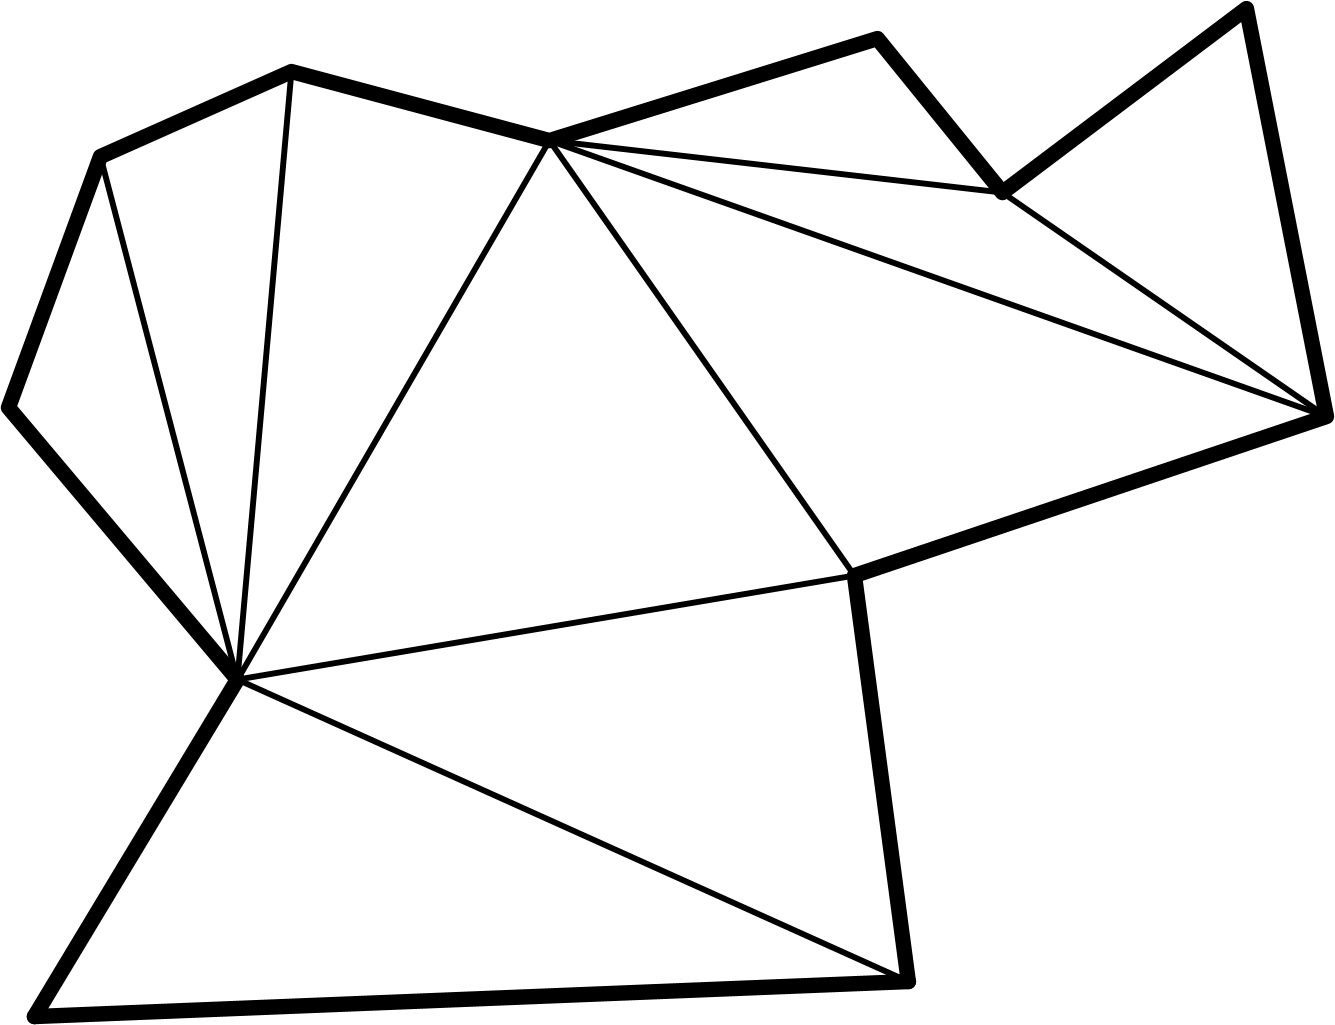
\includegraphics[scale=0.25]{figures/triangulation}
\par\end{center}
\item Pada soal \ref{recursive1} dan \ref{recursive2}, Anda seharusnya
memperhatikan bahwa fungsi-fungsi rekursif lebih lambat daripada padanannya
yang menggunakan perulangan for. Berapa kali lebih lambat? Mengapa
rekursi Fibonacci jauh lebih lambat daripada padanannya yang menggunakan
perulangan for?
\item Misalkan barisan $\left\langle b_{n}\right\rangle $ dan $\left\langle c_{n}\right\rangle $
didefinisikan sebagai berikut.
\begin{eqnarray*}
b_{0} & = & \frac{1}{3};\quad b_{n+1}=4b_{n}-1,\quad n\geq0\\
c_{0} & = & \frac{1}{10};\quad c_{n+1}=4c_{n}(1-c_{n}),\quad n\geq0
\end{eqnarray*}

\begin{enumerate}
\item Tulislah fungsi yang menggunakan perulangan for untuk menghitung suku
$n$ dari barisan $\left\langle b_{n}\right\rangle $. Fungsi Anda
harus memiliki satu argumen, $n$.
\item Tulislah fungsi yang menggunakan perulangan for untuk menghitung suku
$n$ dari barisan $\left\langle c_{n}\right\rangle $. Fungsi Anda
harus memiliki satu argumen, $n$.
\item Tulislah program yang memanggil fungsi Anda dari bagian (a) untuk
menghitung $b_{30}$. Seberapa akurat hasil perhitungan ini? PETUNJUK:
$b_{30}=\frac{1}{3}$. 
\item Tulislah program yang memanggil fungsi Anda dari bagian (b) untuk
menghitung $c_{50}$. Seberapa akurat hasil perhitungan ini? PETUNJUK:
$c_{50}=.5392$, akurat hingga 4 tempat desimal.
\item Dapatkah Anda menemukan cara untuk membuat perhitungan ini lebih andal
(lebih akurat)?
\end{enumerate}
\end{enumerate}
\finishexercises 
